\chapter{Theoretical Fundamentals} % Chapter title

\label{chapter:theoretical_fundamentals} % For referencing the chapter elsewhere, use \ref{chapter:computational_neuro} 

\def \blochwidth {0.3}
\def \histogramwidth {0.5}
\newcommand{\bloch}{\emph{Bloch}-Sphere}
\newcommand{\hgate}{$\mathrm{H}$-Gate}
\newcommand{\xgate}{$\mathrm{X}$-Gate}
\newcommand{\ygate}{$\mathrm{Y}$-Gate}
\newcommand{\zgate}{$\mathrm{Z}$-Gate}
\newcommand{\rygate}{$\mathrm{RY}$-Gate}
\newcommand{\rzgate}{$\mathrm{RZ}$-Gate}
\newcommand{\rxgate}{$\mathrm{RX}$-Gate}
\newcommand{\crygate}{$\mathrm{CRY}$-Gate}
\newcommand{\crzgate}{$\mathrm{CRZ}$-Gate}
\newcommand{\crxgate}{$\mathrm{CRX}$-Gate}

%----------------------------------------------------------------------------------------

\todo{In der Regel ist zumindest ein kurzes The-oriekapitel notwendig. Es nimmt Bezug auf das thematische Oberthema, aber na-türlich nicht auf allgemeine theoretische Grundlagen etwa aus der Naturwissen-schaft.}

\section{Quantum Computing}
Classical computing consists of the infamous 1's and 0's and have for years shaped our world and progress. Quantum computing is, from afar, similar. We have \emph{qubits}, which are synonymous to \emph{bits}, but are fundamentally different. Whereas a bit can only exist in state 0 or 1, a qubit allows us to use any state, be it 0, 1 or a mix of those. Such a mix is referred to as \emph{superposition}. The catch comes when we want to read the value it represents: one cannot directly know the probabilities of measuring 1 or 0 in a qubit.



\begin{figure}[!h]
    \centering
    \tikzset{every picture/.style={line width=0.75pt}} %set default line width to 0.75pt        
    
    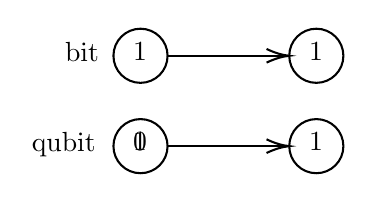
\begin{tikzpicture}[x=0.75pt,y=0.75pt,yscale=-1,xscale=1]
    %uncomment if require: \path (0,300); %set diagram left start at 0, and has height of 300
    
    
    
    % Text Node
    \draw    (117.29, 130) circle [x radius= 13.04, y radius= 13.04]   ;
    \draw (112.29,122) node [anchor=north west][inner sep=0.75pt]   [align=left] {1};
    % Text Node
    \draw    (202, 130) circle [x radius= 13.04, y radius= 13.04]   ;
    \draw (197,122) node [anchor=north west][inner sep=0.75pt]   [align=left] {1};
    % Text Node
    \draw    (202, 173.54) circle [x radius= 13.04, y radius= 13.04]   ;
    \draw (197,165.54) node [anchor=north west][inner sep=0.75pt]   [align=left] {1};
    % Text Node
    \draw (112.29,165.54) node [anchor=north west][inner sep=0.75pt]   [align=left] {0};
    % Text Node
    \draw    (117.29, 173.54) circle [x radius= 13.04, y radius= 13.04]   ;
    \draw (112.29,165.54) node [anchor=north west][inner sep=0.75pt]   [align=left] {1};
    % Text Node
    \draw (79.43,122) node [anchor=north west][inner sep=0.75pt]   [align=left] {bit};
    % Text Node
    \draw (63.43,165.54) node [anchor=north west][inner sep=0.75pt]   [align=left] {qubit};
    % Connection
    \draw    (130.32,173.54) -- (186.96,173.54) ;
    \draw [shift={(188.96,173.54)}, rotate = 180] [color={rgb, 255:red, 0; green, 0; blue, 0 }  ][line width=0.75]    (10.93,-3.29) .. controls (6.95,-1.4) and (3.31,-0.3) .. (0,0) .. controls (3.31,0.3) and (6.95,1.4) .. (10.93,3.29)   ;
    % Connection
    \draw    (130.32,130) -- (186.96,130) ;
    \draw [shift={(188.96,130)}, rotate = 180] [color={rgb, 255:red, 0; green, 0; blue, 0 }  ][line width=0.75]    (10.93,-3.29) .. controls (6.95,-1.4) and (3.31,-0.3) .. (0,0) .. controls (3.31,0.3) and (6.95,1.4) .. (10.93,3.29)   ;
    
    \end{tikzpicture}
    \caption{A comparison of measuring a single bit and a qubit. When measuring the bit, we get the same value that the bit is set to. When measuring a qubit, there is a certain probability of it being 0 and 1, so we measure one of both but don't know the real, intern state of the qubit.}
    \label{figure:comparison_bit_qubit_measurement}
\end{figure}

When measuring a quantum circuit, the qubit states collapse from super positions into the fixed position of 0 or 1. To do additional measurements, the circuit has to be rebuild. Using this data can be collected on the qubit state and a \emph{histogram} constructed, out of which one can calculate the internal probabilities of 1 and 0.

\begin{table}[!h]
    \centering
    \begin{tabular}{|c|c|}
         Measured value & Amount  \\
         \hline
         0 & 547 \\
         1 & 987 \\
    \end{tabular}
    \caption{Table containing all measurements done on a qubit in a superposition. The number of occurrences of a measured 1 or 0 is counted and then used to generate a histogram, as shown in figure \ref{figure:example_histogram}}
    \label{table:example_counts}
\end{table}



\begin{figure}[!h]
    \centering
    \scalebox{\histogramwidth}{
        \includesvg{thesis/Appendices/example_histogram.svg}
    }
    \caption{A histogram generated from the data in table \ref{table:example_counts}, that visually shows the probabilities of 0 and 1. These probabilities can directly be used to visualize the qubits superposition.}
    \label{figure:example_histogram}
\end{figure}

The \emph{Bloch}-Sphere, as shown in figure \ref{figure:basic_bloch_sphere}, is used to further visualize the complex state a qubit is in a 3-dimensional sphere. Using the complex state vector of a \emph{non-entangled} qubit, any superposition can be visualized to show the qubits state.

\begin{figure}[!h]
    \centering
    \scalebox{\blochwidth}{
        \includesvg{thesis/Appendices/Bloch_Sphere_axis.svg}
    }
    \caption{A basic Bloch-Sphere without any visualized state. The axis $x$ and $y$ are annotated accordingly, but the axis $z$ is annotated with $\ket{0}$ and $\ket{1}$ - the states which have a corresponding probability assigned to them. The purple point shows the origin $(0,0,0)$}
    \label{figure:basic_bloch_sphere}
\end{figure}

When measuring a qubit, the state collapses onto the $z$-axis\cite{}, which in turn leads to a measurement of either 0 or 1. Initially, all qubits are set to state $\ket{0}$, which is visualized onto the \emph{Bloch}-Sphere in figure \ref{figure:state_0_bloch_sphere}. A circuit that results in said state is visualized in figure \ref{figure:state_0_circuit}, and its mathematical counterpart in equation \ref{equation:state_0_equation}.

\begin{figure}[!h]
    \centering
    \scalebox{\blochwidth}{
        \includesvg{thesis/Appendices/Bloch_Sphere_state_0.svg}
    }
    \caption{A basic \emph{Bloch}-Sphere with the state $\ket{0}$ visualized onto it.}
    \label{figure:state_0_bloch_sphere}
\end{figure}

\begin{figure}[!h]
    \centering
    \scalebox{1.0}{
    \Qcircuit @C=1.0em @R=1.0em @!R { \\
	 	\nghost{{q} :  } & \lstick{{q} :  } \barrier[0em]{0} & \qw & \qw & \qw\\
	 	\nghost{} & \lstick{} & \ket{\psi_0} &\\
\\ }}
    \caption{A basic circuit consisting of a single qubit $q_0$ that is initially set to $\ket{0}$. The state vector at point $\ket{\psi_0}$ is shown in equation \ref{equation:state_0_equation}.}
    \label{figure:state_0_circuit}
\end{figure}


\begin{equation}
    \centering
    \begin{split}
        \ket{\psi_0} =\ \begin{pmatrix}1 \\ 0\end{pmatrix}\\
    \end{split}
    \label{equation:state_0_equation}
\end{equation}



To create the state $\ket{1}$, the state of the qubit has to be turned by 180° around the $x$ or the $y$ axis. This can be achieved in multiple ways, but the simplest one is the usage of a $\mathbb{X}$-Gate\cite{}. A circuit with such a gate is visualized in figure \ref{figure:x_circuit}, with a \emph{Bloch}-Sphere visualization done in figure \ref{figure:state_1_bloch_sphere}.

\begin{figure}[!h]
    \centering
    \scalebox{\blochwidth}{
        \includesvg{thesis/Appendices/Bloch_Sphere_state_1.svg}
    }
    \caption{A basic \emph{Bloch}-Sphere with the state $\ket{1}$ visualized onto it.}
    \label{figure:state_1_bloch_sphere}
\end{figure}

\begin{figure}[!h]
    \centering\scalebox{1.0}{
    \Qcircuit @C=1.0em @R=0.2em @!R { \\
	 	\nghost{{q} :  } & \lstick{{q} :  } \barrier[0em]{0} & \qw & \gate{\mathrm{X}} \barrier[0em]{0} & \qw & \qw & \qw\\
	 	\nghost{} & \lstick{} & \ket{\psi_0} & & \ket{\psi_1} &\\
\\ }}
    \caption{Caption}
    \label{figure:x_circuit}
\end{figure}


\begin{equation}
    \centering
    \begin{split}
        \ket{\psi_1} =\ \mathrm{X}\ket{\psi_0} =\ \begin{pmatrix} 0 & 1\\ 1 & 0\end{pmatrix}\begin{pmatrix}1 \\ 0\end{pmatrix} =\ \begin{pmatrix}0 \\ 1 \end{pmatrix}\\
    \end{split}
    \label{equation:state_1_equation}
\end{equation}

The state $\ket{\psi_1}$ can be directly calculated with the $\mathrm{X}$-Gate and $\ket{0}$, which results in state $\ket{1}$, as demonstrated in equation \ref{equation:state_1_equation}. Whilst their definitions are not equal, the gates $\mathrm{Y}$\cite{} and $\mathrm{Z}$\cite{} also apply a full 180° rotation around their corresponding axes. \par

The \emph{Hadamard}-Gate, or $\mathrm{H}$-Gate, can be used to quickly create a superposition of a single qubit where the state $\ket{0}$ and $\ket{1}$ have the same probability (so, 0.5) of being measured.

\begin{figure}[!h]
    \centering\scalebox{1.0}{
    \Qcircuit @C=1.0em @R=0.2em @!R { \\
	 	\nghost{{q} :  } & \lstick{{q} :  } \barrier[0em]{0} & \qw & \gate{\mathrm{H}} \barrier[0em]{0} & \qw & \qw & \qw\\
	 	\nghost{} & \lstick{} & \ket{\psi_0} & & \ket{\psi_1} &\\
\\ }}
    \caption{Caption}
    \label{figure:h_circuit}
\end{figure}

\begin{equation}
    \centering
    \begin{split}
        \ket{\psi_1} =\ \mathrm{H}\ket{\psi_0} =\ \frac{1}{\sqrt{2}}\begin{pmatrix} 1 & 1 \\ 1 & -1 \end{pmatrix}\begin{pmatrix}1 \\ 0\end{pmatrix} =\ \frac{1}{\sqrt{2}}\begin{pmatrix}1 \\ 0 \end{pmatrix} + \frac{1}{\sqrt{2}}\begin{pmatrix}0 \\ 1 \end{pmatrix}\\
    \end{split}
    \label{equation:equal_superposition_equation}
\end{equation}

\begin{figure}[!h]
    \centering
    \scalebox{\blochwidth}{
        \includesvg{thesis/Appendices/Bloch_Sphere_state_0_1_equal.svg}
    }
    \caption{A basic \emph{Bloch}-Sphere with the state $\frac{1}{\sqrt{2}}\begin{pmatrix}1 \\ 0 \end{pmatrix} + \frac{1}{\sqrt{2}}\begin{pmatrix}0 \\ 1 \end{pmatrix}$ visualized onto it.}
    \label{figure:state_0_bloch_sphere}
\end{figure}

To assess that the visualization, and the described behaviour of qubits is correct, these assumptions can be evaluated the formal way. When calculating the to be expected probability of a certain state, the Hermitian transposition\cite{} is used. Equation \ref{equation:basic_h_measurement} demonstrates the calculation of the probabilities the \hgate\ assigns to the measurements of $0$ and $1$.

\begin{equation}
    \centering
    \begin{split}
        \ket{\psi_1} &=\ \frac{1}{\sqrt{2}}\ket{0} + \frac{1}{\sqrt{2}}\ket{1}\\
        \bra{0}\ket{\psi_1} &=\ \frac{1}{\sqrt{2}}\begin{pmatrix}1 & 0 \end{pmatrix}\begin{pmatrix}1 \\ 0 \end{pmatrix} + \frac{1}{\sqrt{2}}\begin{pmatrix}1 & 0 \end{pmatrix}\begin{pmatrix}0 \\ 1 \end{pmatrix} \\
        \bra{0}\ket{\psi_1} &=\ \frac{1}{\sqrt{2}}\\
        |\bra{0}\ket{\psi_1}|^2 &=\ 0.5\\
        |\bra{1}\ket{\psi_1}|^2 &=\ \left|\frac{1}{\sqrt{2}}\right|^2 =\ 0.5\\
    \end{split}
    \label{equation:basic_h_measurement}
\end{equation}

As shown, both states $\ket{0}$ and $\ket{1}$ have the same probability of $0.5$. When desiring probabilities that are not equal for both states, there are gates the likes of \rygate\cite{}, \rxgate\cite{} and \rzgate\cite{}. These gates allow the rotation around the corresponding axes by a parameter that can be supplied. To create a circuit that achieves the probabilities from the histogram, \ref{figure:example_histogram}, the usage of these are needed. Equation \ref{equation:rx_gate_definition} shows the definition of the \rxgate.

\begin{equation}
    \centering
    \begin{split}
        \mathrm{RX}(\theta) =\ \begin{pmatrix} \cos{\frac{\theta}{2}}   & -i\sin{\frac{\theta}{2}} \\
        -i\sin{\frac{\theta}{2}} & \cos{\frac{\theta}{2}}
    \end{pmatrix}
    \end{split}
    \label{equation:rx_gate_definition}
\end{equation}

The formal definition used in equation \ref{equation:basic_h_measurement} as well as the \rygate\ can be combined to calculate the parameters needed to achieve the probabilities shown in \ref{figure:example_histogram}, as demonstrated in equation \ref{equation:parameter_from_probabilities}. 

\begin{equation}
    \centering
    \begin{split}
        |\bra{1}\ket{\psi_1}|^2 &=\ 0.643 \\
        \begin{pmatrix}1 & 0\end{pmatrix}\ket{\psi_1} &=\ \sqrt{0.643} \\
        \ket{\psi_1} &=\ \sqrt{0.357}\begin{pmatrix} 1 \\ 0\end{pmatrix} + \sqrt{0.643}\begin{pmatrix} 0 \\ 1\end{pmatrix}\\
        \ket{\psi_1} &=\ \begin{pmatrix}\sqrt{0.643}\\ \sqrt{0.357}\end{pmatrix}\\
        \mathrm{RY}(\theta)\ket{0} &=\ \begin{pmatrix}\sqrt{0.357}\\ \sqrt{0.643}\end{pmatrix} \\
        \begin{pmatrix}\cos{\frac{\theta}{2}} \\ -i\sin{\frac{\theta}{2}}\end{pmatrix} &=\ \begin{pmatrix}\sqrt{0.357}\\ \sqrt{0.643}\end{pmatrix}\\
        \theta_{cos} &=\ 2(\acos{\sqrt{0.357}}) =\ 1.8608\\
        \theta_{sin} &=\ 2(\asin{\sqrt{0.643}}) =\ 1.8608\\
        \theta &=\ \theta_{sin} =\ \theta_{cos}\\
    \end{split}
    \label{equation:parameter_from_probabilities}
\end{equation}

With the value for $\theta$ calculated, the circuit from figure \ref{figure:circuit_for_histogram} is designed and evaluated to comparet it to the histogram from \ref{figure:example_histogram} to the one in figure \ref{figure:circuit_histogram}.

\begin{figure}
    \centering
    \scalebox{1.0}{
    \Qcircuit @C=1.0em @R=0.2em @!R { \\
    	 	\nghost{{q} :  } & \lstick{{q} :  } & \gate{\mathrm{R_Y}\,(\mathrm{1.8608})} & \qw & \qw\\
    \\ }}
    \caption{Caption}
    \label{figure:circuit_for_histogram}
\end{figure}


\begin{figure}[!h]
    \centering
    \scalebox{\histogramwidth}{
        \includesvg{thesis/Appendices/calculated_circuit_histogram.svg}
    }
    \caption{A histogram generated from the data in table \ref{table:example_counts}, that visually shows the probabilities of 0 and 1. These probabilities can directly be used to visualize the qubits superposition.}
    \label{figure:circuit_histogram}
\end{figure}

%%%%%%%%%%%%%%%%%%%%%%%%%%%%%%%%%%%%%%

\newpage

\section{Multiple Query Optimization}

A query\cite{codd_relational_1970} is a demand for information to be pulled from a database. Such a query can vary in size and structure, as well as in execution time. These are often written in the query language \code{SQL}, which is often adapted to the corresponding software\cite{shirgoldbird_microsoft_nodate}\cite{the_postgresql_global_development_group_postgresql_2022} it executes on. 

    
\begin{figure}[!h]
    \centering
    \begin{minted}{sql}
        SELECT * FROM USERS u
        WHERE u.NAME = "Abraham"
    \end{minted}
    \caption{This example SQL code would tell the database we want all data from table \emph{USER}, where the name equals \emph{Abraham}}
    \label{figure:sql_query_example}
\end{figure}

The example query in figure \ref{figure:sql_query_example} is parsed, and the resulting query plan used to retrieve and display data that is saved in the database. Table \ref{table:sql_query_result_example} resembles the result of such a query.

\begin{table}[!h]
    \centering
    \begin{tabular}{|c|c|c|}
        \hline
        Name    & Surname & Gender \\ \hline
        Abraham & Martin  & M      \\ \hline
        Abraham & Tart    & F      \\ \hline
    \end{tabular}
    \caption{Exemplary data returned after executing the SQL query from figure \ref{figure:sql_query_example}, where the first row resembles the name of the attributes in the column}
    \label{table:sql_query_result_example}
\end{table}

Before any execution takes place, the queries themselves are parsed into multiple execution plans\cite{microsoft_execution_nodate}. These plans usually resemble the same operations, just in a different order – this can result in precious time savings. In a large system that handles multiple requests per second, these plans can be used to combine certain sub-sequences of a plan and therefore save execution time\cite{roy_multi-query_2009}. This by itself has been proven to be an \emph{NP-Hard} problem\cite{}. Nevertheless, finding the fastest combination of all plans can be done classically with an exhaustive algorithm in $O(n^2)$\footnote{Assuming that the number of queries and plans per query are equal, if not, then the runtime is $O(P^Q)$, where $P$ is the number of plans per query, and $Q$ the total number of queries}. There exist classical proposals that are faster than $O(n^2)$\cite{}, that whilst not finding the fastest combination, deliver results that still offer acceptable speed up. Hybrid approach combinations use QAOA (short for Quantum Approximate Optimization Algorithm)\cite{} have shown to be quasi-optimal solution finders with a runtime of $O(I \cdot (PQ)^2)$.\par

\subsection{Query Dissection}
A query can be dissected into a variety of plans that can be executed to get the data in the desired format. Figure \ref{figure:query_with_plans} shows a query, which has two differing plans.

\begin{figure}[!h]
    \centering
    \tikzset{every picture/.style={line width=0.75pt}} %set default line width to 0.75pt        
    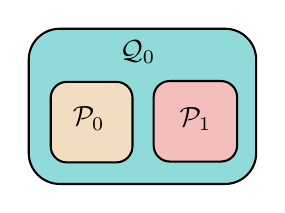
\begin{tikzpicture}[x=0.75pt,y=0.75pt,yscale=-1,xscale=1]
        %uncomment if require: \path (0,300); %set diagram left start at 0, and has height of 300
        %Rounded Rect [id:dp08144411333317714] 
        \draw  [fill={rgb, 255:red, 144; green, 218; blue, 217 }  ,fill opacity=1 ] (80.2,130.56) .. controls (80.2,122.3) and (86.9,115.6) .. (95.16,115.6) -- (174.84,115.6) .. controls (183.1,115.6) and (189.8,122.3) .. (189.8,130.56) -- (189.8,175.44) .. controls (189.8,183.7) and (183.1,190.4) .. (174.84,190.4) -- (95.16,190.4) .. controls (86.9,190.4) and (80.2,183.7) .. (80.2,175.44) -- cycle ;
        %Rounded Rect [id:dp5870651506756062] 
        \draw  [fill={rgb, 255:red, 242; green, 221; blue, 192 }  ,fill opacity=1 ] (90.8,148.96) .. controls (90.8,144.67) and (94.27,141.2) .. (98.56,141.2) -- (122.44,141.2) .. controls (126.73,141.2) and (130.2,144.67) .. (130.2,148.96) -- (130.2,172.24) .. controls (130.2,176.53) and (126.73,180) .. (122.44,180) -- (98.56,180) .. controls (94.27,180) and (90.8,176.53) .. (90.8,172.24) -- cycle ;
        %Rounded Rect [id:dp7624346816043626] 
        \draw  [fill={rgb, 255:red, 243; green, 190; blue, 188 }  ,fill opacity=1 ] (140.4,148.56) .. controls (140.4,144.27) and (143.87,140.8) .. (148.16,140.8) -- (172.84,140.8) .. controls (177.13,140.8) and (180.6,144.27) .. (180.6,148.56) -- (180.6,171.84) .. controls (180.6,176.13) and (177.13,179.6) .. (172.84,179.6) -- (148.16,179.6) .. controls (143.87,179.6) and (140.4,176.13) .. (140.4,171.84) -- cycle ;
        % Text Node
        \draw (151.4,152.2) node [anchor=north west][inner sep=0.75pt]   [align=left] {$\displaystyle \mathcal{P}_{1}$};
        % Text Node
        \draw (100,151.8) node [anchor=north west][inner sep=0.75pt]   [align=left] {$\displaystyle \mathcal{P}_{0}$};
        % Text Node
        \draw (122.8,119.8) node [anchor=north west][inner sep=0.75pt]   [align=left] {$\displaystyle \mathcal{Q}_{0}$};
    \end{tikzpicture}
    \caption{A query that can be executed through two different plans, which end up delivering the same result but might offer potential time savings.}
    \label{figure:query_with_plans}
\end{figure}

The plans themselves consist of many different instructions, which can be as simple as loading a table from storage into memory or searching a certain table for a given value. If one were to add another query that is to be executed parallel to the one in figure \ref{figure:query_with_plans}, overlapping instructions could be combined so that they're executed exactly once, and then reused for both plans, as shown in figure \ref{figure:plan_tree}. Each instruction in any plan consist of single operations applied to tables of the database that are based on relational algebra\cite{codd_relational_1970}\footnote{But not limited to them, as modern databases also include hashing and indexing in the plans. None the less, these operations can also be combined to save previous runtime}. It is easy to imagine that, depending on the environment at hand, single operations will happen plenty of times in parallel. Putting into perspective the number of users that modern applications\cite{uber_technologies_inc_uber_2022} can have, finding shortcuts in plans does not only reduce execution time but saves money and improves customer experience.

\begin{figure}[!h]
    \centering
\tikzset{every picture/.style={line width=0.75pt}} %set default line width to 0.75pt        

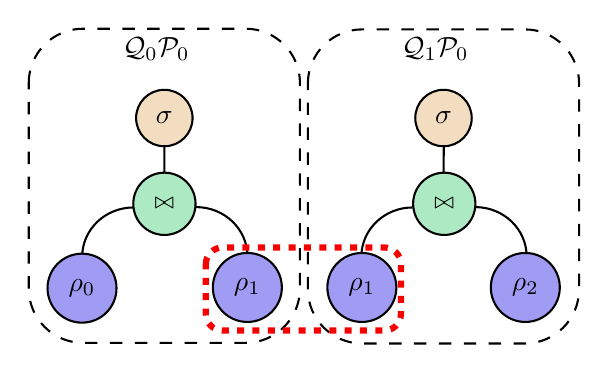
\begin{tikzpicture}[x=0.75pt,y=0.75pt,yscale=-1,xscale=1]
%uncomment if require: \path (0,300); %set diagram left start at 0, and has height of 300

%Rounded Rect [id:dp3098689700784747] 
\draw  [dash pattern={on 4.5pt off 4.5pt}] (120.33,155.05) .. controls (120.33,140.62) and (132.03,128.92) .. (146.47,128.92) -- (224.87,128.92) .. controls (239.3,128.92) and (251,140.62) .. (251,155.05) -- (251,254.12) .. controls (251,268.55) and (239.3,280.25) .. (224.87,280.25) -- (146.47,280.25) .. controls (132.03,280.25) and (120.33,268.55) .. (120.33,254.12) -- cycle ;
%Shape: Arc [id:dp8469571253916317] 
\draw  [draw opacity=0] (146.09,238.65) .. controls (146.2,225.59) and (157.23,215.04) .. (170.82,215.04) -- (170.82,238.86) -- cycle ; \draw   (146.09,238.65) .. controls (146.2,225.59) and (157.23,215.04) .. (170.82,215.04) ;  
%Shape: Arc [id:dp8173590455021038] 
\draw  [draw opacity=0] (201,214.86) .. controls (214.66,214.86) and (225.73,225.52) .. (225.73,238.67) -- (201,238.67) -- cycle ; \draw   (201,214.86) .. controls (214.66,214.86) and (225.73,225.52) .. (225.73,238.67) ;  
%Straight Lines [id:da6630213040029864] 
\draw    (185.68,199.4) -- (185.67,186) ;
%Rounded Rect [id:dp5436966787626745] 
\draw  [dash pattern={on 4.5pt off 4.5pt}] (254.83,155.38) .. controls (254.83,140.95) and (266.53,129.25) .. (280.97,129.25) -- (359.37,129.25) .. controls (373.8,129.25) and (385.5,140.95) .. (385.5,155.38) -- (385.5,254.45) .. controls (385.5,268.88) and (373.8,280.58) .. (359.37,280.58) -- (280.97,280.58) .. controls (266.53,280.58) and (254.83,268.88) .. (254.83,254.45) -- cycle ;
%Shape: Arc [id:dp13654717695684715] 
\draw  [draw opacity=0] (280.59,238.65) .. controls (280.7,225.59) and (291.73,215.04) .. (305.32,215.04) -- (305.32,238.86) -- cycle ; \draw   (280.59,238.65) .. controls (280.7,225.59) and (291.73,215.04) .. (305.32,215.04) ;  
%Shape: Arc [id:dp7676498647138272] 
\draw  [draw opacity=0] (335.5,214.86) .. controls (349.16,214.86) and (360.23,225.52) .. (360.23,238.67) -- (335.5,238.67) -- cycle ; \draw   (335.5,214.86) .. controls (349.16,214.86) and (360.23,225.52) .. (360.23,238.67) ;  
%Straight Lines [id:da7192788563309687] 
\draw    (320.18,199.4) -- (320.33,184.44) ;
%Rounded Rect [id:dp6770297453454031] 
\draw  [color={rgb, 255:red, 246; green, 1; blue, 1 }  ,draw opacity=1 ][dash pattern={on 2.53pt off 3.02pt}][line width=2.25]  (205.67,242.33) .. controls (205.67,237.92) and (209.25,234.33) .. (213.67,234.33) -- (291.67,234.33) .. controls (296.08,234.33) and (299.67,237.92) .. (299.67,242.33) -- (299.67,266.33) .. controls (299.67,270.75) and (296.08,274.33) .. (291.67,274.33) -- (213.67,274.33) .. controls (209.25,274.33) and (205.67,270.75) .. (205.67,266.33) -- cycle ;

% Text Node
\draw (164.17,131.65) node [anchor=north west][inner sep=0.75pt]    {$\mathcal{Q}_{0}\mathcal{P}_{0}$};
% Text Node
\draw  [fill={rgb, 255:red, 242; green, 221; blue, 192 }  ,fill opacity=1 ]  (185.67, 171.95) circle [x radius= 13.6, y radius= 13.6]   ;
\draw (185.67,171.95) node    {$\sigma $};
% Text Node
\draw (298.67,131.65) node [anchor=north west][inner sep=0.75pt]    {$\mathcal{Q}_{1}\mathcal{P}_{0}$};
% Text Node
\draw  [fill={rgb, 255:red, 242; green, 221; blue, 192 }  ,fill opacity=1 ]  (320.17, 171.95) circle [x radius= 13.6, y radius= 13.6]   ;
\draw (320.17,171.95) node    {$\sigma $};
% Text Node
\draw  [fill={rgb, 255:red, 173; green, 234; blue, 195 }  ,fill opacity=1 ]  (185.71, 213.28) circle [x radius= 15, y radius= 15]   ;
\draw (185.71,213.28) node  [font=\footnotesize]  {$\bowtie $};
% Text Node
\draw  [fill={rgb, 255:red, 173; green, 234; blue, 195 }  ,fill opacity=1 ]  (320.54, 213.28) circle [x radius= 15, y radius= 15]   ;
\draw (320.54,213.28) node  [font=\footnotesize]  {$\bowtie $};
% Text Node
\draw  [fill={rgb, 255:red, 160; green, 156; blue, 243 }  ,fill opacity=1 ]  (146.01, 253.92) circle [x radius= 16.62, y radius= 16.62]   ;
\draw (146.01,253.92) node   [align=left] {$\displaystyle \rho _{0}$};
% Text Node
\draw  [fill={rgb, 255:red, 160; green, 156; blue, 243 }  ,fill opacity=1 ]  (225.67, 253.58) circle [x radius= 16.62, y radius= 16.62]   ;
\draw (225.67,253.58) node   [align=left] {$\displaystyle \rho _{1}$};
% Text Node
\draw  [fill={rgb, 255:red, 160; green, 156; blue, 243 }  ,fill opacity=1 ]  (280.84, 253.58) circle [x radius= 16.62, y radius= 16.62]   ;
\draw (280.84,253.58) node   [align=left] {$\displaystyle \rho _{1}$};
% Text Node
\draw  [fill={rgb, 255:red, 160; green, 156; blue, 243 }  ,fill opacity=1 ]  (359.59, 253.58) circle [x radius= 16.62, y radius= 16.62]   ;
\draw (359.59,253.58) node   [align=left] {$\displaystyle \rho _{2}$};


\end{tikzpicture}


    \caption{Two differing plans $\mathcal{Q}_0\mathcal{P}_0$ and $\mathcal{Q}_1\mathcal{P}_1$, which serve different goals but contain the same operation $\rho_1$, marked in the red dotted box}
    \label{figure:plan_tree}
\end{figure}

Figure \ref{figure:plan_tree} shows two different queries that contain the same sub-operation $\rho_b$. The operation can be used by both queries, which means we do not have to execute it twice. 

Plans, costs and savings can be mathematically expressed. Let there be $\mathcal{C}$, a given function which returns the cost for a given operation or collection of operations as defined in equation \ref{equation:formal_cost_function}. Let there also be a given function $\mathcal{S}$, which calculates the savings two collections of operations can achieve, as shown in equation \ref{equation:formal_savings_function}.

\begin{equation}
    \centering
    \begin{split}
        \mathcal{C}(\mathcal{Q}_0\mathcal{P}_1) =\ 45 \\
        \mathcal{C}(\rho_1) =\ 15 \\
    \end{split}
    \label{equation:formal_cost_function}
\end{equation}

\begin{equation}
    \centering
    \begin{split}
        \mathcal{S}(\mathcal{Q}_0\mathcal{P}_1, \mathcal{Q}_1\mathcal{P}_0) =\ 15 \\
        \mathcal{S}(\mathcal{Q}_0\mathcal{P}_0, \mathcal{Q}_1\mathcal{P}_1) =\ 0 \\
    \end{split}
    \label{equation:formal_savings_function}
\end{equation}


Taking a problem consisting of two queries $\mathcal{Q}_0$ and $\mathcal{Q}_1$, each of which has two plans $\mathcal{P}_0$ and $\mathcal{P}_1$, we can calculate the total costs of running them collectively as shown in equation \ref{equation:formal_total_cost_calculation}.

\begin{equation}
    \centering
    \begin{split}
        \mathcal{C}(\mathcal{Q}_0\mathcal{P}_0) + \mathcal{C}(\mathcal{Q}_1\mathcal{P}_0) - \mathcal{S}(\mathcal{Q}_0\mathcal{P}_0, \mathcal{Q}_1\mathcal{P}_0) \\
        \mathcal{C}(\mathcal{Q}_0\mathcal{P}_0) + \mathcal{C}(\mathcal{Q}_1\mathcal{P}_1) - \mathcal{S}(\mathcal{Q}_0\mathcal{P}_0, \mathcal{Q}_1\mathcal{P}_1) \\
        \mathcal{C}(\mathcal{Q}_0\mathcal{P}_1) + \mathcal{C}(\mathcal{Q}_1\mathcal{P}_0) - \mathcal{S}(\mathcal{Q}_0\mathcal{P}_1, \mathcal{Q}_1\mathcal{P}_0) \\
        \mathcal{C}(\mathcal{Q}_0\mathcal{P}_1) + \mathcal{C}(\mathcal{Q}_1\mathcal{P}_1) - \mathcal{S}(\mathcal{Q}_0\mathcal{P}_1, \mathcal{Q}_1\mathcal{P}_1) \\
    \end{split}
    \label{equation:formal_total_cost_calculation}
\end{equation}

If we change the problem space from two queries to more, or create an uneven number of plans per query, the complexity starts to rise sharply.



\newpage
